\begin{frame}{Motivación}
  \begin{block}{¿Cuál es el verdadero impacto de un derrame de petróleo?}
    \begin{itemize}
      \item Consecuencias ambientales
      \item Consecuencias sociales
      \item Consecuencias económicas
    \end{itemize}
  \end{block}

\end{frame}

\begin{frame}{Pozos perforados (2011 - 2013)}
    \begin{figure}
        \centering
        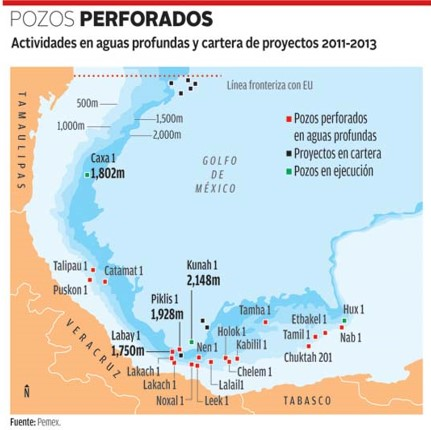
\includegraphics[scale=0.4]{img/section_01/pozos_perforados_2013.jpg}
        \caption{Actividades de exploración y perforación en 2013}
        \label{fig:section_01_pozos}
    \end{figure}
\end{frame}

\begin{frame}{Infraestructura Petrolera 2015)}
    \begin{figure}
        \centering
        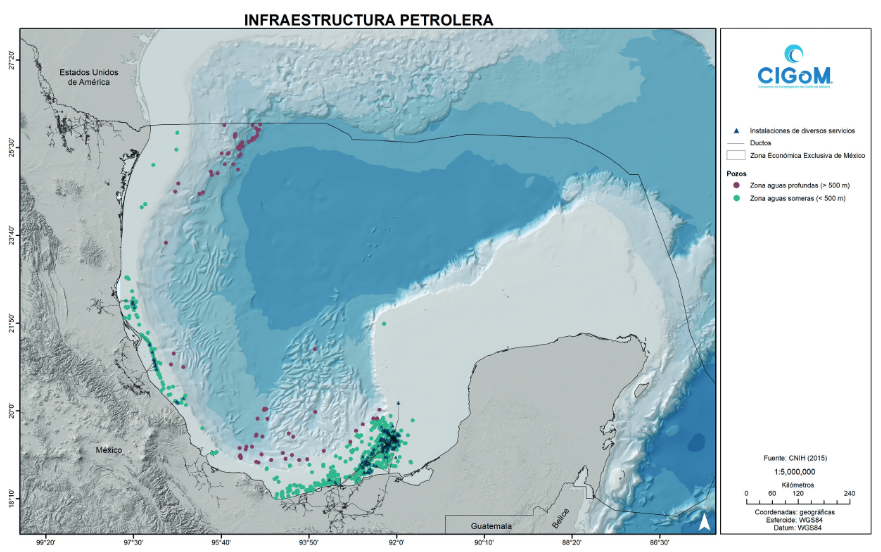
\includegraphics[scale=0.3]{img/section_01/infraestructura_petrolera}
        \caption{Infraestructura petrolera de exploración, extracción y producción de gas petróleo en la Zona Económica Exclusiva mexicana. Fuente: Atlas de Línea Base Ambiental del Golfo de México, Tomo IV, CIGOM}
        \label{fig:section_01_infraestructura}
    \end{figure}
\end{frame}

\begin{frame}{Deep Water Horizon}
    \begin{figure}
        \centering
        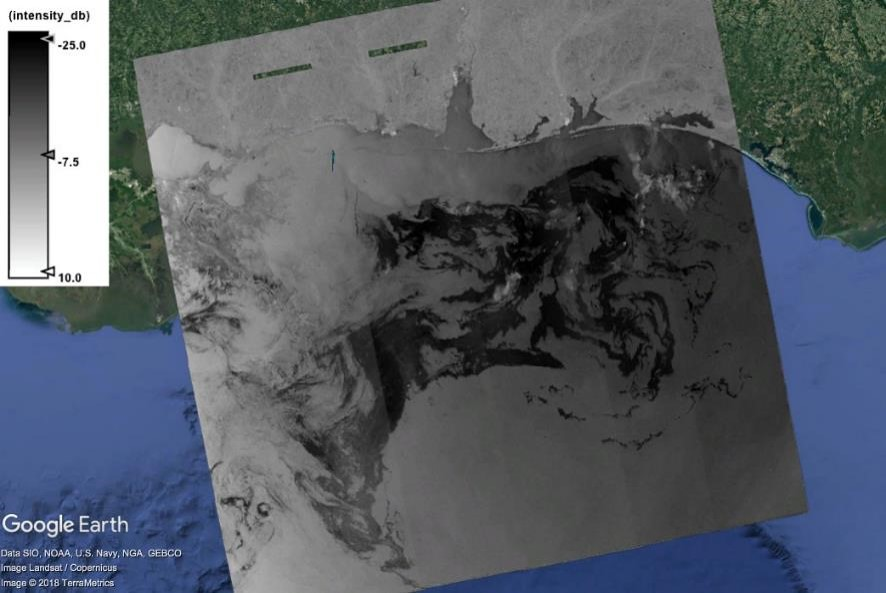
\includegraphics[scale=0.3]{img/section_01/deep-water-horizon.jpg}
        \caption{Extensión del derrame}
        \label{fig:section_01_deep_water_horizon}
    \end{figure}

    Estimación del derrame: 779,000 toneladas de crudo.
\end{frame}

\begin{frame}{Deep Water Horizon - Timelime}
  \begin{figure}
    \centering
    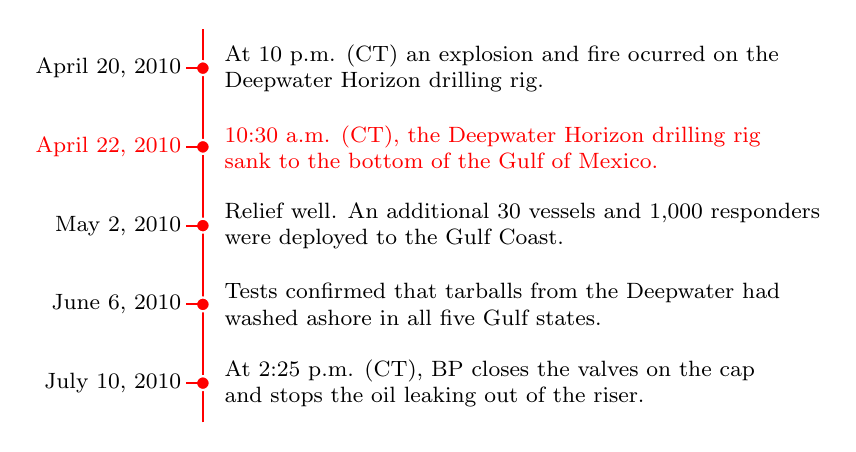
\begin{tikzpicture}[scale=0.5,every node/.style={outer sep=5pt}]
      %Notation: {year, the title of the event}
      %NOTE! Everyting is zero-based
      \footnotesize
      \def\ourInfo{{
        {"April 20, 2010","At 10 p.m. (CT) an explosion and fire ocurred on the \\ Deepwater Horizon drilling rig."},
        {"April 22, 2010","10:30 a.m. (CT), the Deepwater Horizon drilling rig \\ sank to the bottom of the Gulf of Mexico."},
        {"May 2, 2010","Relief well. An additional 30 vessels and 1,000 responders \\were deployed to the Gulf Coast."},
        {"June 6, 2010","Tests confirmed that tarballs from the Deepwater had \\washed ashore in all five Gulf states."},
        {"July 10, 2010","At 2:25 p.m. (CT), BP closes the valves on the cap \\and stops the oil leaking out of the riser."}
      }}
      \pgfmathsetmacro{\length}{4}% Zero based.

      % Loop through the array containing all events.
      \foreach \i in {0, ..., \length}{
          \pgfmathsetmacro{\year}{\ourInfo[\i][0]}% Get the left cell (year)
          \pgfmathsetmacro{\eventName}{\ourInfo[\i][1]}% Get the right cell (event name)
          \draw[thick,red] (0,-2*\i-2)--(0,-2*\i);% Draw vertical line
          \ifnum \i=1 % Should be in red text
            \draw(0,-2*\i-1) node[red, right, align = left]{\eventName};% Display the event name
            \draw(0,-2*\i-1) node[red, left] {\year};
          \else % Should be in black text
             \draw(0,-2*\i-1) node[right, black, align = left]{\eventName};% Display the event name
             \draw(0,-2*\i-1) node[left] {\year};% Display the year
          \fi
      }
      % Draw the bullet with the dash
      \foreach \i in {0, ..., \length}{
          \filldraw[draw = white, fill = red,thick] (0,-2*\i-1) circle (5pt);
          \draw[thick,red] (-12pt,-2*\i-1)--(0,-2*\i-1);
      }
    \end{tikzpicture}
    \caption{Línea de tiempo del evento. Fuente: \url{https://response.restoration.noaa.gov/timelines/10-years-ago-deepwater-horizon-oil-spill}}
  \end{figure}
  \footnotesize
  \footnote{}
\end{frame}

\begin{frame}{Ixtoc I}    
    \begin{figure}
        \centering
        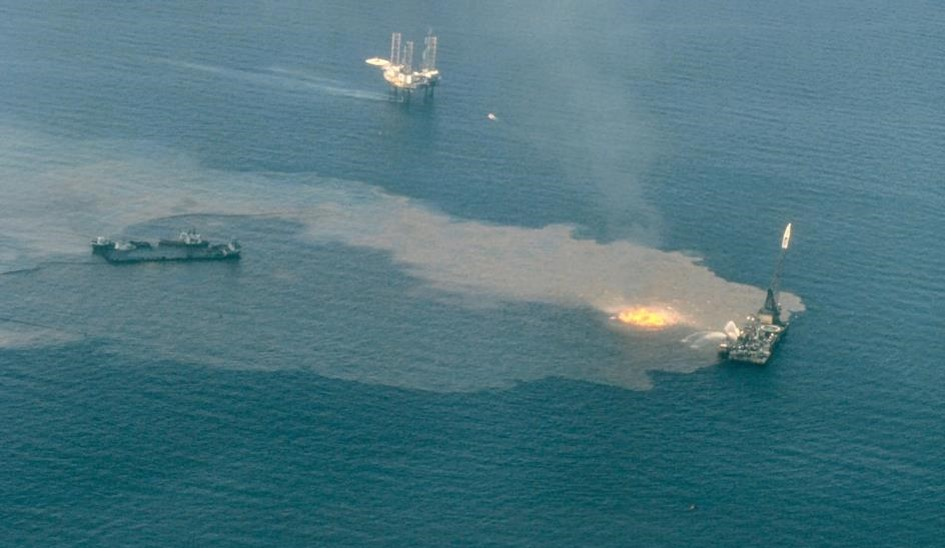
\includegraphics[scale=0.3]{img/section_01/explosion_ixtoc.jpg}
        \caption{Explosión del pozo Ixtoc I, Sonda de Campeche, 3 de junio de 1979}
        \label{fig:section_01_explosion_ixtoc}
    \end{figure}

    Estimación del derrame, 530,000 toneladas de crudo.
\end{frame}

\begin{frame}{Ek Balam}    
    \begin{figure}
        \centering
            \begin{tabular}[c]{cc}
              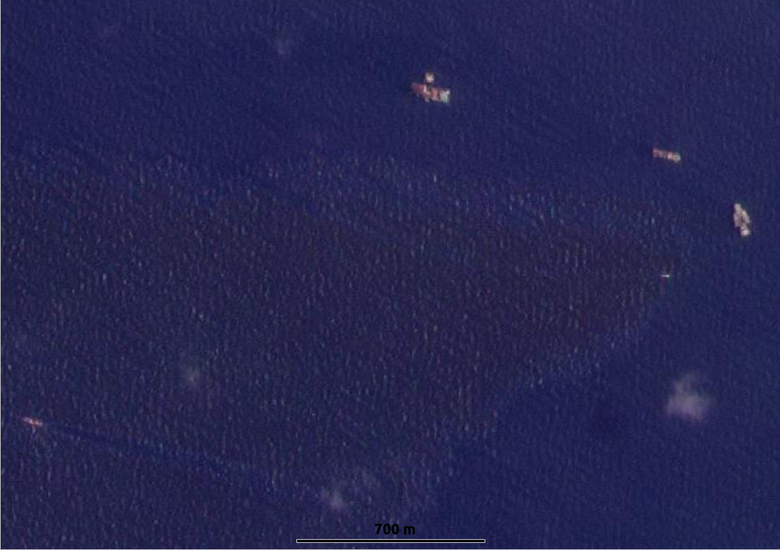
\includegraphics[scale=0.2]{img/section_01/ek_balam-6-julio.png}&
              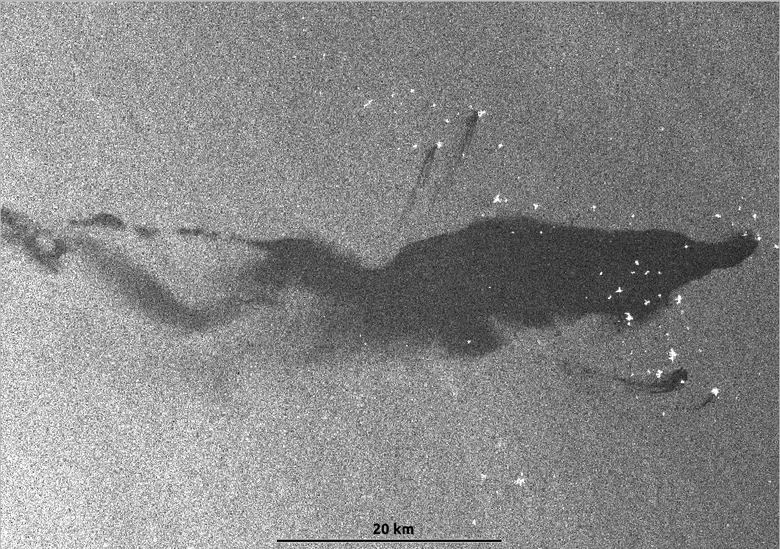
\includegraphics[scale=0.2]{img/section_01/ek_balam-12-julio.png}\\
            \end{tabular}
        \caption{Derrame en la Sonda de Campeche, Julio 2023}
        \label{fig:section_01_explosion_ixtoc}
    \end{figure}
\end{frame}

\begin{frame}{Dinámica de la interacción océano-petróleo}
    \footnotesize
    \begin{block}{Diferentes procesos físicos y químicos dificultan el tratamiento}
      \begin{itemize}
        \item Dispersión
        \item Evaporación
        \item Emulsión
        \item Sedimentación
      \end{itemize}
    \end{block}
    \begin{figure}
      \centering
      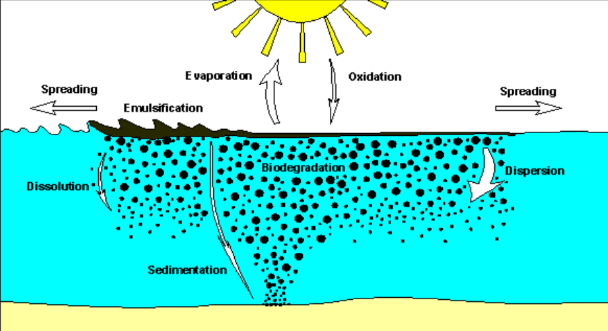
\includegraphics[scale=0.3]{img/section_01/dinamica-derrame.png}
      \caption{Dinámica de la interacción}
      \label{fig:section_01_dinamica_derrame}
    \end{figure}    
\end{frame}
